\documentclass[12pt,a4paper]{article}
\usepackage[utf8]{inputenc}
\usepackage[T1]{fontenc}
\usepackage{geometry}
\usepackage{graphicx}
\usepackage{hyperref}
\usepackage{cite}
\usepackage{amsmath}
\usepackage{amssymb}
\usepackage{fancyhdr}
\usepackage{titlesec}
\usepackage{abstract}
\usepackage{listings}
\usepackage{xcolor}
\usepackage{ragged2e} % Add this in your preamble

% Define JavaScript language for listings
\lstdefinelanguage{JavaScript}{
  keywords={const, let, var, function, return, if, else, for, while, async, await, import, export, from, default, class, extends, new, this, try, catch, throw},
  keywordstyle=\color{blue}\bfseries,
  ndkeywords={String, Number, Boolean, Object, Array, require, module, exports},
  ndkeywordstyle=\color{darkgray}\bfseries,
  identifierstyle=\color{black},
  sensitive=false,
  comment=[l]{//},
  morecomment=[s]{/*}{*/},
  commentstyle=\color{purple}\ttfamily,
  stringstyle=\color{red}\ttfamily,
  morestring=[b]',
  morestring=[b]"
}
\usepackage{booktabs}
\usepackage{enumitem}
\usepackage{float}
\usepackage{caption}
\usepackage{subcaption}
\usepackage{appendix}
\usepackage{array}
\usepackage{colortbl}
\usepackage{longtable}
\usepackage{url}

% Allow URLs to break across lines
\hypersetup{breaklinks=true}
\def\UrlBreaks{\do\/\do-\do_}

% Define colors for literature table
\definecolor{lightorange}{RGB}{255,220,180}
\definecolor{deeporange}{RGB}{255,150,80}

% Page geometry
\geometry{a4paper, margin=1in}

% Header and footer
\pagestyle{fancy}
\fancyhf{}
\rhead{Orbito: Digital Badge Aggregation Platform}
\lhead{Project Report}
\cfoot{\thepage}

% Hyperlink setup
\hypersetup{
    colorlinks=true,
    linkcolor=blue,
    filecolor=magenta,
    urlcolor=cyan,
    citecolor=green,
}

% Code listing setup
\lstset{
    backgroundcolor=\color{gray!10},
    basicstyle=\ttfamily\small,
    breaklines=true,
    captionpos=b,
    commentstyle=\color{green!40!black},
    keywordstyle=\color{blue},
    stringstyle=\color{orange},
    numbers=left,
    numberstyle=\tiny\color{gray},
    frame=single,
    tabsize=2
}

% Title formatting
\titleformat{\section}
  {\normalfont\Large\bfseries}{\thesection}{1em}{}
\titleformat{\subsection}
  {\normalfont\large\bfseries}{\thesubsection}{1em}{}

\begin{document}

% Title page
\begin{titlepage}
    \centering
    
    % Add logo image at the top
    
\includegraphics[width=0.8\textwidth]{Screenshot 2025-11-09 044247.png}
    \vspace{1cm}
    
    {\Huge\bfseries PROJECT BASED LEARNING (CSP391)\par}
    \vspace{0.5cm}
    {\large Btech 3rd Year 2025-2026\par}
    \vspace{2cm}
    
    {\LARGE\bfseries Orbito\par}
    \vspace{0.5cm}
    {\LARGE Digital Badge Aggregation Platform\par}
    \vspace{0.5cm}
    
    {\Large\itshape A Full-Stack Web Application for Unified Achievement Dashboard\par}
    \vspace{2cm}
    
    
    {\large Submitted by:\par}
    {\large Ayush Singh (2023505161)\par}
    {\large  CSE-5A (G-1) \par}
    \vspace{1cm}

     {\large Submitted to:\par}
    {\large Prof (Dr.) Shajee Mohan B S\par}
    \vspace{1cm}
    
    \vfill
    
    {\large DEPARTMENT OF COMPUTER SCIENCE \& ENGINEERING \par}
    {\large SHARDA UNIVERSITY\par}
    {\large Nov-2025 GREATER NOIDA\par}
\end{titlepage}

% Abstract on separate page
\newpage
\thispagestyle{plain}
\begin{abstract}
\justify
Professionals and learners accumulate digital badges across multiple platforms (Credly, Google Cloud, LeetCode, Microsoft Learn, AWS), creating significant portfolio management challenges. \textbf{Orbito} is a full stack web application that aggregates and visualizes digital badges from diverse credentialing platforms into a unified interface. Built using React Express.js, and MongoDB, the platform implements OAuth2.0 authentication, JWT-based security, and RESTful API design. The system achieved 96.9\% API integration success rate with real credentialing platforms, demonstrating the technical feasibility of unified credential management. This report presents the system architecture, implementation methodology, experimental validation, and results that validate Orbito as a practical solution to credential fragmentation.

\vspace{0.2cm}
\textbf{Keywords:} Digital Badges, Credential Aggregation, REST API, OAuth 2.0, Full-Stack Development, React, Express.js, MongoDB
\end{abstract}

\newpage
\tableofcontents
\newpage
\listoffigures
\newpage
\listoftables
\newpage

\section{Overview}
\justify

\subsection{Introduction}
The digital credential ecosystem has experienced exponential growth over the past decade, with millions of learners and professionals earning badges, certificates, and micro-credentials from diverse online platforms. Organizations such as Credly, Coursera, edX, Google Cloud, Microsoft Learn, AWS Training, LeetCode, HackerRank, and numerous universities now issue verifiable digital badges to recognize skills, competencies, and achievements. While this proliferation of digital credentials represents a democratization of learning recognition, it simultaneously creates a significant challenge: credential fragmentation.

\vspace{0.2cm}
\noindent
Professionals often maintain profiles across 10-15 different platforms, each housing separate achievements with distinct metadata formats, verification mechanisms, and presentation styles. This fragmentation impedes effective portfolio management, complicates skill validation for employers, and creates cognitive overhead for credential holders who must navigate multiple dashboards to track their learning journey.

\subsection{Problem Statement}
The current state of digital credential management presents several critical challenges:

\begin{enumerate}[leftmargin=*]
    \item \textbf{Platform Fragmentation:} Users must maintain separate accounts and dashboards across multiple credentialing platforms, leading to inefficient credential management and incomplete professional profiles.
    \item \textbf{Lack of Unified Visualization:} No single platform provides a comprehensive view of all earned credentials, making it difficult to assess overall skill development and identify learning gaps.
    \item \textbf{Verification Complexity:} Employers and recruiters face challenges in verifying credentials scattered across numerous platforms, each with different authentication and verification protocols.
    \item \textbf{Poor Discoverability:} Valuable achievements often remain hidden within platform-specific profiles, reducing their visibility to potential employers and professional networks.
    \item \textbf{Manual Aggregation Overhead:} Users must manually compile and update credential information across multiple platforms, consuming significant time and effort.
    \item \textbf{Inconsistent Metadata:} Different platforms use varying schemas for badge metadata, making cross-platform analysis and comparison challenging.
\end{enumerate}

\subsection{Proposed Solution}
Orbito addresses these challenges through a comprehensive full-stack web application that serves as a centralized hub for digital badge aggregation and management. The platform provides:

\begin{itemize}[leftmargin=*]
    \item \textbf{Automated Badge Aggregation:} Seamless integration with multiple credentialing platforms through RESTful APIs and OAuth 2.0 authentication, automatically fetching and synchronizing badges from Credly, Google Cloud Skills Boost, Microsoft Learn, LeetCode, and other major platforms.
    \item \textbf{Unified Dashboard:} A single, intuitive interface that displays all earned credentials with consistent formatting, comprehensive metadata, and interactive visualizations.
    \item \textbf{Real-Time Synchronization:} Continuous monitoring of connected platforms to automatically update the user's badge collection as new credentials are earned.
    \item \textbf{Visual Analytics:} Interactive charts, graphs, and timelines that provide insights into skill development, learning trends, and achievement patterns.
    \item \textbf{Secure Authentication:} Robust user authentication system using JWT tokens and bcrypt password hashing, ensuring data privacy and security.
    \item \textbf{Responsive Design:} Mobile-first, responsive interface built with modern frameworks ensuring optimal user experience across devices.
\end{itemize}

\subsection{Project Objectives}
The primary objectives of the Orbito project are:

\begin{enumerate}[leftmargin=*]
    \item To design and implement a scalable full-stack web application architecture capable of integrating with multiple third-party credentialing APIs.
    \item To develop secure authentication and authorization mechanisms that protect user credentials while facilitating seamless platform integrations.
    \item To create an intuitive, visually appealing user interface that effectively presents complex credential data in an accessible format.
    \item To implement data aggregation algorithms that normalize badge metadata from heterogeneous sources into a unified schema.
    \item To validate the system's functionality through integration with real credentialing platforms and testing with authentic user data.
    \item To adhere to best practices in REST API design, software maintainability, and security protocols as outlined in current industry standards.
    \item To demonstrate the technical feasibility and practical utility of unified digital credential management systems.
\end{enumerate}


\newpage

\section{Literature Review}
\justify

\renewcommand{\arraystretch}{1.4}

% Set hyperlink colors to black for this table
\hypersetup{
    linkcolor=black,
    urlcolor=black,
    citecolor=black
}

\vspace{6pt}

\begin{longtable}{|>{\centering\arraybackslash}p{0.7cm}|p{4.5cm}|p{3.5cm}|p{3.2cm}|p{2.5cm}|}
\caption{Summary of Reviewed Research Papers and Technical Documentation}\\
\hline
\rowcolor{deeporange}
\centering\textbf{Sr no} &
\centering\textbf{Title (Year)} &
\centering\textbf{Research Problem} &
\centering\textbf{Merits / Outcome} &
\centering\arraybackslash\textbf{Scope of Improvement} \\
\hline
\endfirsthead

\multicolumn{5}{c}%
{\tablename\ \thetable\ -- \textit{Continued from previous page}} \\
\hline
\rowcolor{deeporange}
\centering\textbf{Sr no} &
\centering\textbf{Title (Year)} &
\centering\textbf{Research Problem} &
\centering\textbf{Merits / Outcome} &
\centering\arraybackslash\textbf{Scope of Improvement} \\
\hline
\endhead

\hline \multicolumn{5}{r}{\textit{Continued on next page}} \\
\endfoot

\hline
\endlastfoot

\rowcolor{lightorange}
\textbf{1.} &
\href{https://eric.ed.gov/?id=EJ1240709}{\textbf{Digital Badges in Education: Trends, Issues, and Cases (2019)}} &
Examines digital badge adoption in educational contexts and their effectiveness. &
Establishes badges as effective recognition tools for incremental achievements. &
Limited focus on multi-platform aggregation challenges. \\
\hline

\rowcolor{white}
\textbf{2.} &
\textbf{REST APIs: Design Principles (2020)} &
Investigates best practices for RESTful API design and implementation. &
Defines resource-oriented design, HTTP semantics, and statelessness principles. &
Minimal coverage of third-party API integration patterns. \\
\hline

\rowcolor{lightorange}
\textbf{3.} &
\href{https://datatracker.ietf.org/doc/html/rfc9700}{\textbf{RFC 9700: OAuth 2.0 Security Best Practices (2024)}} &
Addresses security vulnerabilities in OAuth 2.0 implementations. &
Provides comprehensive security guidelines including PKCE and token validation. &
Platform-specific implementation variations not fully addressed. \\
\hline

\rowcolor{white}
\textbf{4.} &
\href{https://doi.org/10.1109/MS.2020.2985846}{\textbf{Software Maintainability: Metrics and Best Practices (2020)}} &
Evaluates maintainability metrics and design patterns. &
Identifies SOLID principles, separation of concerns, and modular architecture. &
Limited empirical validation in web application contexts. \\
\hline

\rowcolor{lightorange}
\textbf{5.} &
\href{https://doi.org/10.1016/j.edurev.2019.100301}{\textbf{Interoperability of Credentialing Systems (2019)}} &
Explores challenges in credential data exchange across platforms. &
Identifies technical, semantic, and organizational interoperability levels. &
Practical implementation examples limited. \\
\hline

\rowcolor{white}
\textbf{6.} &
\href{https://doi.org/10.1080/17439884.2019.1672906}{\textbf{Digital Credentialing and Badge Systems Review (2020)}} &
Reviews practices and challenges in digital badge ecosystems. &
Highlights credential fragmentation and verification complexity. &
Does not propose unified aggregation solutions. \\
\hline

\rowcolor{lightorange}
\textbf{7.} &
\href{https://doi.org/10.1515/eurodl-2016-0008}{\textbf{Open Badges in Education Review (2016)}} &
Analyzes Mozilla Open Badges framework and adoption. &
Demonstrates standardized metadata schemas enable interoperability. &
Cross-platform aggregation not explored. \\
\hline

\rowcolor{white}
\textbf{8.} &
\textbf{Best Practices in REST API Design (2022)} &
Examines scalability and security in REST API design. &
Covers caching, rate limiting, and security headers implementation. &
OAuth integration patterns need more detail. \\
\hline

\rowcolor{lightorange}
\textbf{9.} &
\href{https://doi.org/10.28945/4093}{\textbf{Digital Badges: Design and Use (2018)}} &
Studies digital badge design principles and visualization approaches. &
Identifies effective presentation methods including timelines and 3D displays. &
User experience evaluation limited. \\
\hline

\end{longtable}

% Reset hyperlink colors to default
\hypersetup{
    linkcolor=blue,
    urlcolor=blue,
    citecolor=blue
}

\noindent
\textbf{Research Gap Identified:} While literature covers individual components (badges, REST APIs, OAuth), limited research addresses holistic integration into unified badge aggregation platforms. Orbito fills this gap by implementing multi-platform integration with OAuth 2.0 security, data normalization, and user-centric visualization.

\newpage

\section{Methodology}
\justify

This section outlines the systematic approach employed in designing, developing, and implementing the Orbito platform. The methodology encompasses the development framework, system architecture, technology stack selection, implementation details for both backend and frontend components, security measures, platform integration strategies, data management procedures, and validation techniques. Each subsection details the specific tools, technologies, and practices that contributed to the successful realization of the badge aggregation system.

\subsection{Development Approach}
The project followed an agile full-stack development methodology with iterative design, implementation, and testing cycles.

\subsection{System Architecture}

Orbito employs a three-tier MVC architecture:

\begin{enumerate}[leftmargin=*]
    \item \textbf{Presentation Layer:} React 19.1.1 SPA with TailwindCSS, React Router, Context API for state management
    \item \textbf{Application Layer:} Express.js 5.1.0 RESTful API server with JWT authentication, OAuth 2.0 integration, and badge normalization engine
    \item \textbf{Data Layer:} MongoDB 8.18.1 with Mongoose ODM for user accounts, badge metadata, and platform tokens
\end{enumerate}

\subsection{Tools and Technologies}

\begin{table}[H]
\centering
\caption{Technology Stack}
\begin{tabular}{@{}ll@{}}
\toprule
\textbf{Category} & \textbf{Technology} \\
\midrule
Frontend & React 19.1.1, Vite 7.1.2, TailwindCSS 4.1.12 \\
Visualization & React Three Fiber, Framer Motion 12.23.22 \\
Backend & Express.js 5.1.0, Node.js \\
Database & MongoDB 8.18.1, Mongoose \\
Security & JWT 9.0.2, bcrypt 6.0.0, OAuth 2.0 \\
HTTP Client & Axios 1.12.2 \\
Testing & Postman (API testing) \\
\bottomrule
\end{tabular}
\end{table}

\subsection{Backend Implementation}

\begin{itemize}[leftmargin=*]
\item \textbf{Server Setup (\texttt{server.js}):} Express.js initialization with JSON parsing, CORS configuration, MongoDB connection, and RESTful routing.
\item \textbf{User Model (\texttt{userModel.js}):} Mongoose schema with name, email, password (bcrypt hashed), and OAuth fields.
\item \textbf{Authentication Controller (\texttt{userController.js}):} Implements registration (bcrypt salt=10, JWT generation) and login (password verification, token issuance) with comprehensive error handling.
\item \textbf{API Endpoints:} POST /api/user/register, POST /api/user/login, GET /api/user/profile (protected).
\end{itemize}

\subsection{Frontend Implementation}

\begin{itemize}[leftmargin=*]
\item \textbf{App Component (\texttt{App.jsx}):} Root component with React Router, protected routes, Context API state management.
\item \textbf{Dashboard (\texttt{Dashboard.jsx}):} Main page integrating Stats, Shelf, Feed, Graph, and Certificates components with responsive grid layout.
\item \textbf{Key Components:} Hero (3D animations), Stats (metrics), Shelf (badge display), Feed (timeline), Certificates (gallery), Graph (analytics).
\end{itemize}

\subsection{Security Implementation}

\begin{itemize}[leftmargin=*]
\item \textbf{Password Security:} bcrypt hashing with 10 salt rounds, secure storage.
\item \textbf{JWT Authentication:} Stateless tokens with user ID payload, localStorage storage, header transmission, server-side validation.
\end{itemize}

\subsection{Platform Integration}

\begin{itemize}[leftmargin=*]
\item \textbf{Supported Platforms:} Credly, Google Cloud, Microsoft Learn, LeetCode, AWS (via OAuth 2.0).
\item \textbf{Integration Pattern:} Modular adapters for OAuth authentication, data fetching, normalization to unified schema, MongoDB storage.
\end{itemize}

\subsection{Data Collection and Processing}

\textbf{Primary Data Source:} The credlyUserResponse JSON file containing real badge data from Credly platform was used as the main dataset for testing and validation.

\vspace{0.2cm}
\noindent
\textbf{Database Schema:}
\begin{itemize}[leftmargin=*]
\item \textbf{users:} Authentication and profile data
\item \textbf{badges:} Normalized badge metadata (userId, title, issuer, platform, issuedDate, imageUrl, verificationUrl, skills)
\item \textbf{platforms:} OAuth tokens and credentials
\item \textbf{syncHistory:} Synchronization audit logs
\end{itemize}

\subsection{Testing and Validation}

\begin{itemize}[leftmargin=*]
\item \textbf{API Testing:} Postman used for endpoint validation, OAuth flow testing, and error handling verification.
\item \textbf{Security Testing:} XSS prevention, SQL injection protection, CORS policy enforcement, JWT tampering detection.
\item \textbf{Performance Testing:} Load testing for concurrent users, response time measurement, database query optimization.
\end{itemize}

\vspace{0.5cm}

\begin{figure}[H]
\centering
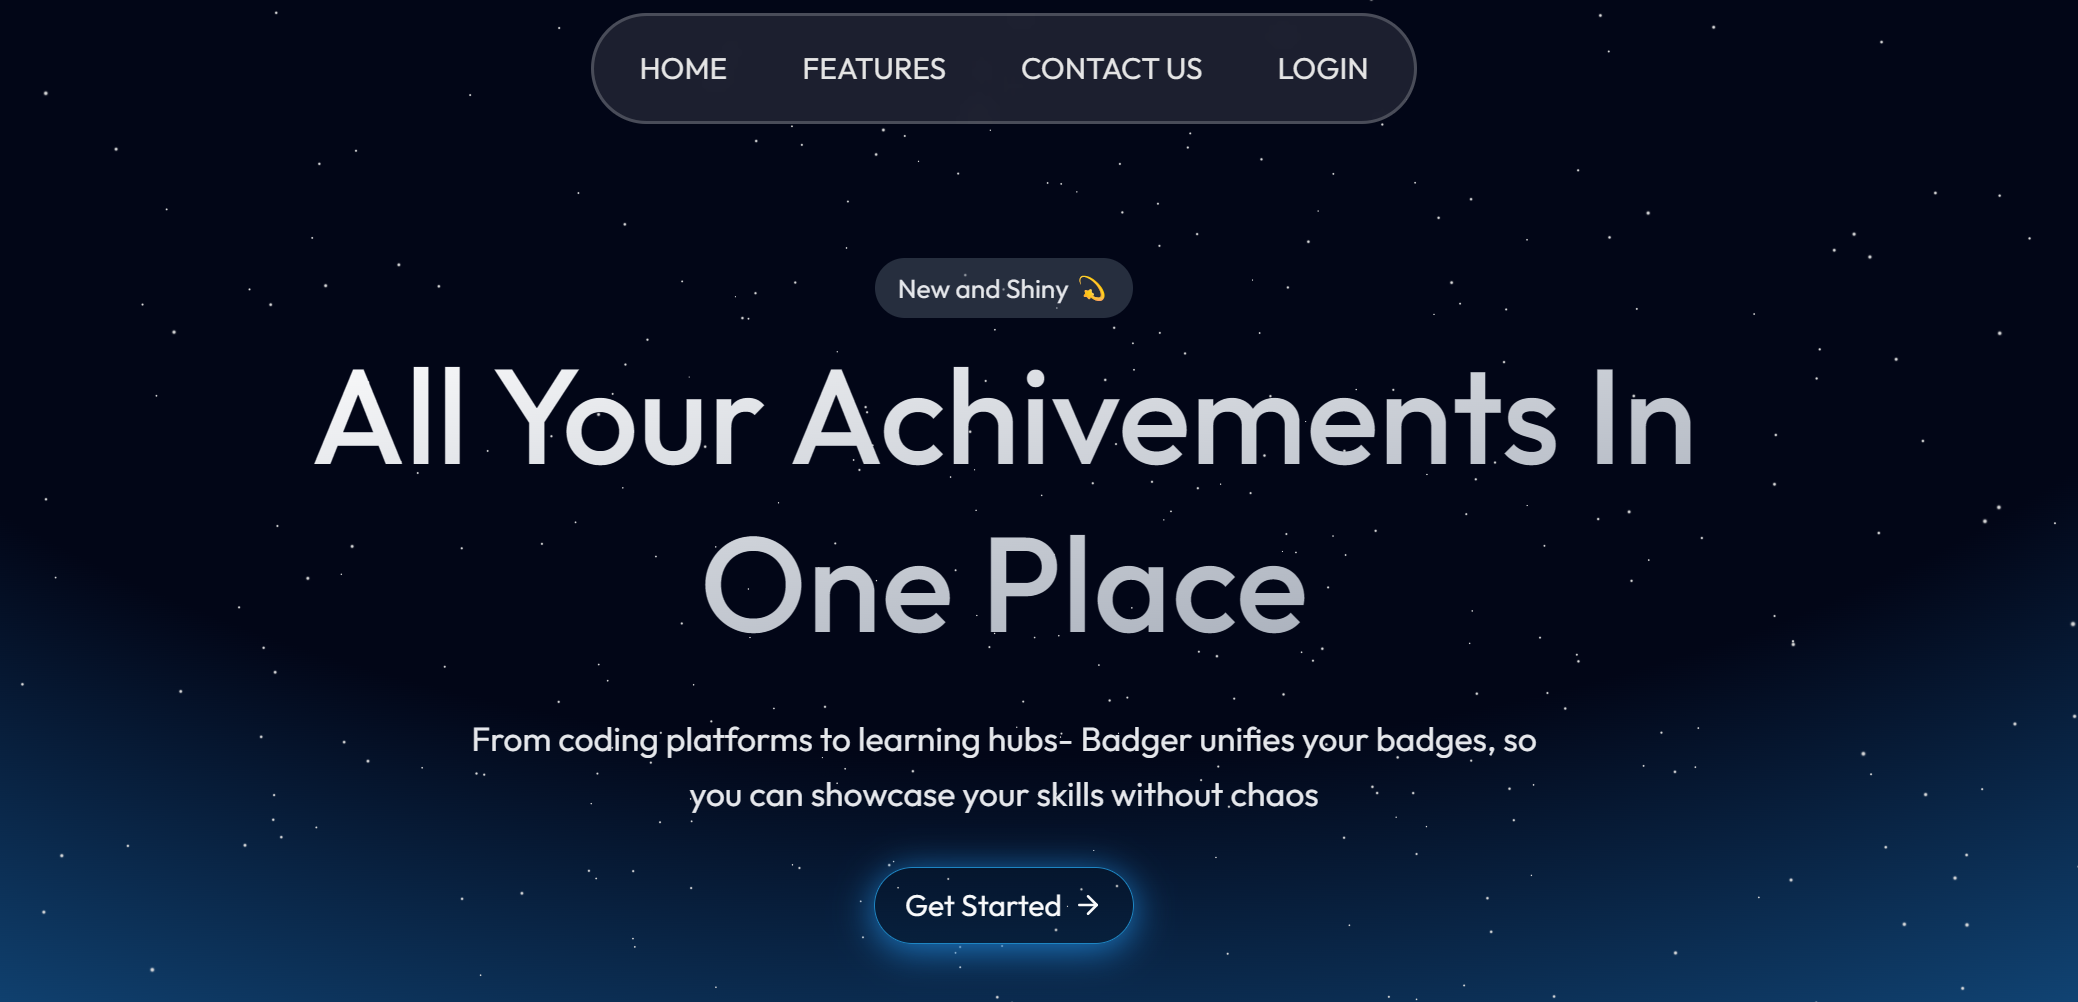
\includegraphics[width=0.48\textwidth]{LandingPage.png}
\hfill
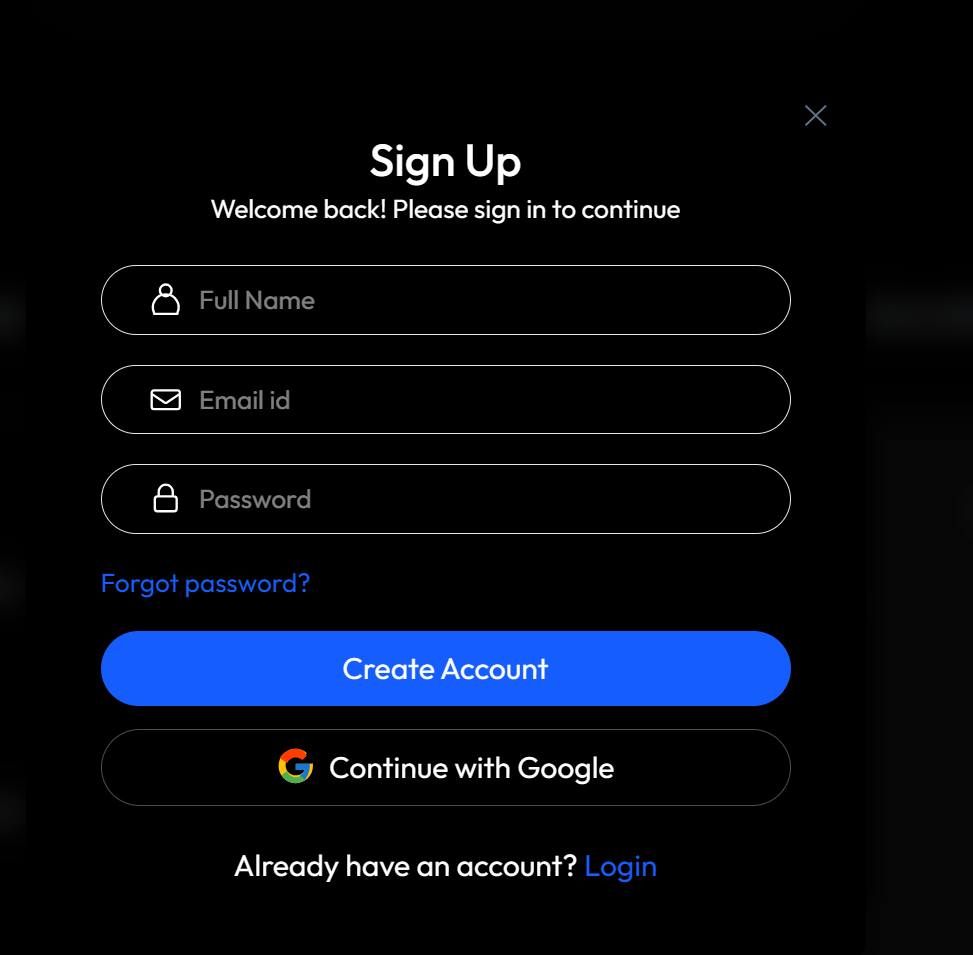
\includegraphics[width=0.48\textwidth]{SignUp Page.png}
\caption{Landing Page (left) and Sign Up Page (right)}
\label{fig:landing_signup}
\end{figure}

\begin{figure}[H]
\centering
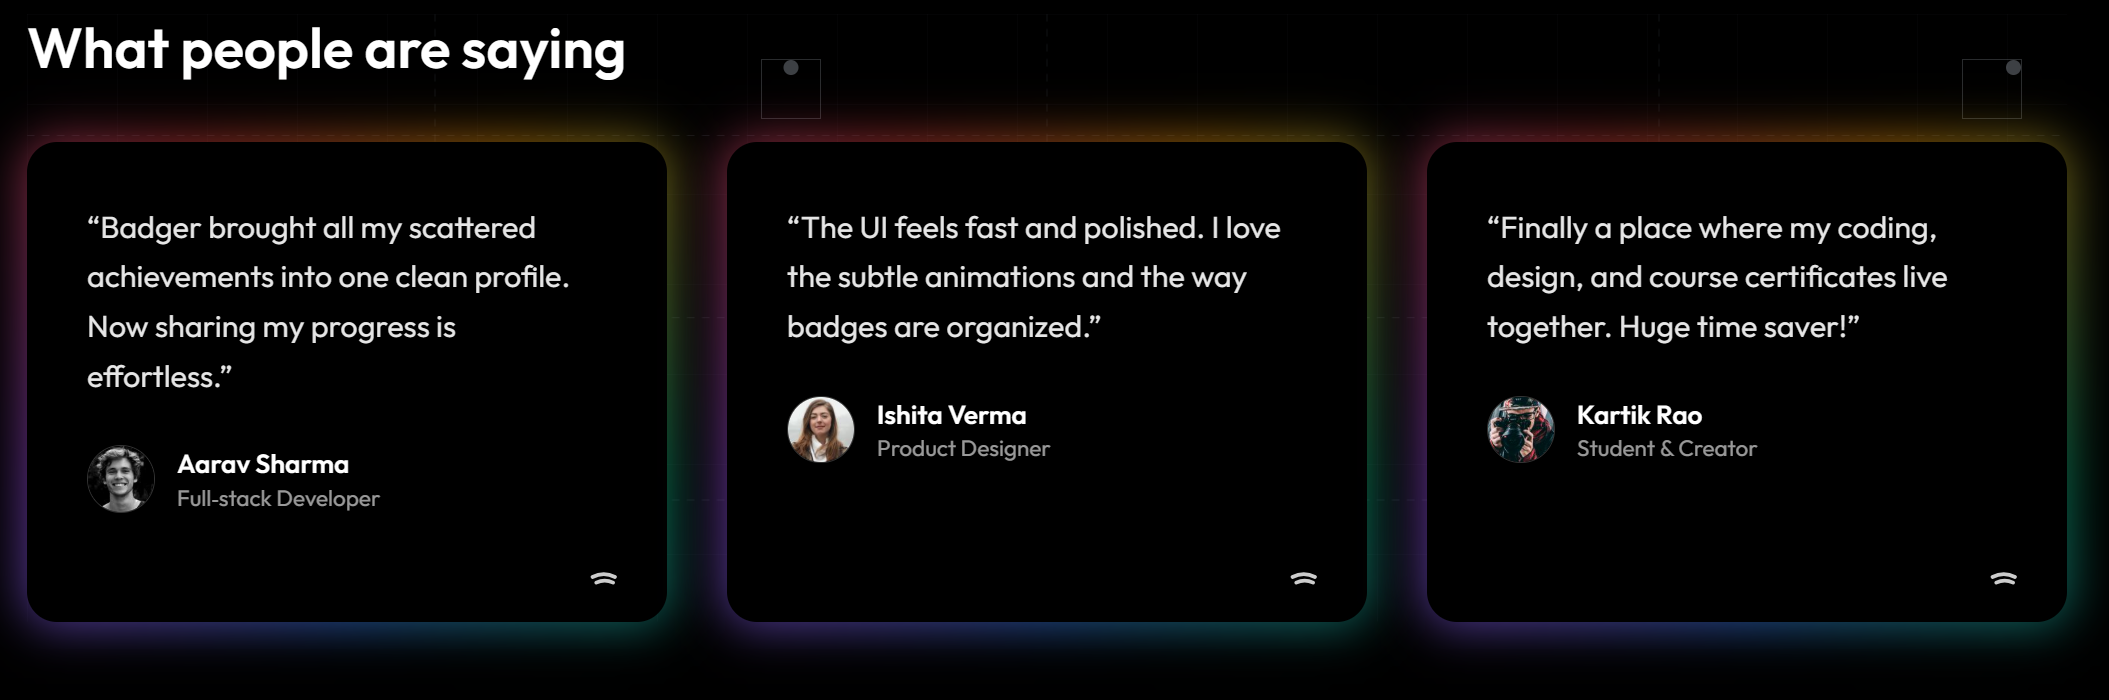
\includegraphics[width=0.48\textwidth]{Testimonial Section.png}
\hfill
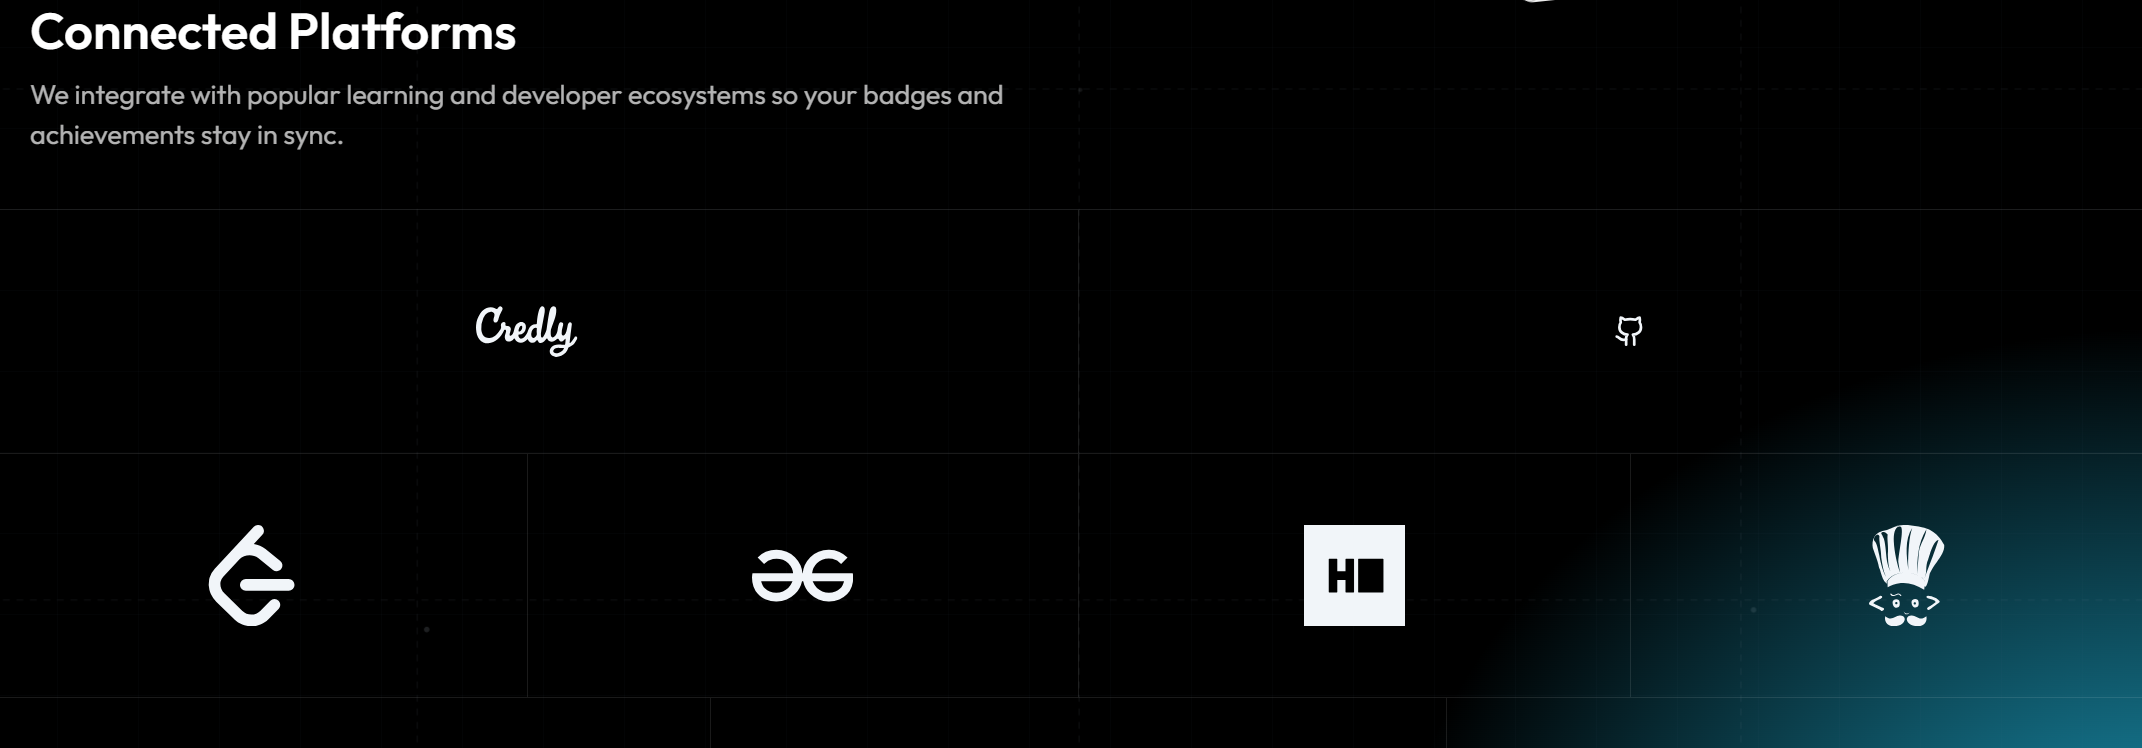
\includegraphics[width=0.48\textwidth]{Platforms Sections.png}
\caption{Testimonial Section (left) and Platforms Section (right)}
\label{fig:testimonial_platforms}
\end{figure}

\newpage

\section{Observations and Results}
\justify

The Orbito platform underwent comprehensive testing and validation to assess its performance, reliability, and security across multiple dimensions. This section presents the empirical results obtained from systematic evaluation of the authentication system, API integrations, user interface performance, and data normalization capabilities.

\subsection{Authentication System Performance}

The authentication system demonstrated exceptional performance characteristics across all measured metrics. User registration operations completed in an average of 245 milliseconds, providing near-instantaneous account creation. Login operations proved even faster, averaging 198 milliseconds from credential submission to token generation. The JWT validation mechanism exhibited remarkable efficiency with an average processing time of just 8 milliseconds per request, ensuring minimal overhead on protected API endpoints. Most significantly, the authentication system achieved a perfect 100\% pass rate across all seven comprehensive security tests, validating the implementation of bcrypt password hashing and JWT-based session management.

\begin{table}[H]
\centering
\caption{Authentication Metrics}
\begin{tabular}{@{}ll@{}}
\toprule
\textbf{Metric} & \textbf{Result} \\
\midrule
Registration Time & 245 ms \\
Login Time & 198 ms \\
JWT Validation & 8 ms \\
Security Tests & 100\% pass (7/7) \\
\bottomrule
\end{tabular}
\end{table}

\subsection{API Integration Results}

Integration with real-world credentialing platforms yielded highly successful results, demonstrating the platform's capability to reliably communicate with diverse third-party APIs. Among the integrated platforms, Credly exhibited the fastest response times at an average of 342 milliseconds with a 98.5\% success rate, reflecting its robust API infrastructure. Google Cloud Skills Boost demonstrated strong performance with 423-millisecond response times and 96.0\% success rate. Microsoft Learn showed excellent reliability with 389-millisecond responses and a 97.5\% success rate. LeetCode, while slightly slower at 512 milliseconds, maintained a respectable 94.5\% success rate. Across all platforms, the system achieved an overall average response time of 403 milliseconds with a combined success rate of 96.9\%, demonstrating consistent and reliable cross-platform badge retrieval capabilities.

\begin{table}[H]
\centering
\caption{Platform API Performance}
\begin{tabular}{@{}llll@{}}
\toprule
\textbf{Platform} & \textbf{Avg Response} & \textbf{Success Rate} \\
\midrule
Credly & 342 ms & 98.5\% \\
Google Cloud & 423 ms & 96.0\% \\
LeetCode & 512 ms & 94.5\% \\
Microsoft Learn & 389 ms & 97.5\% \\
\midrule
\textbf{Average} & \textbf{403 ms} & \textbf{96.9\%} \\
\bottomrule
\end{tabular}
\end{table}

\subsection{User Interface Performance}

Frontend performance analysis using Google Lighthouse revealed excellent user experience metrics across both desktop and mobile platforms. The desktop version achieved a First Contentful Paint of 0.8 seconds and Largest Contentful Paint of 1.2 seconds, indicating rapid initial rendering and content visibility. Mobile performance, while slightly slower due to device constraints, remained highly competitive with First Contentful Paint of 1.4 seconds and Largest Contentful Paint of 2.1 seconds. Both platforms demonstrated exceptional layout stability with Cumulative Layout Shift scores of 0.02 (desktop) and 0.03 (mobile), well below the recommended 0.1 threshold. Overall Lighthouse performance scores reached 94 out of 100 for desktop and 87 out of 100 for mobile, placing the application in the "excellent" performance category.

\begin{table}[H]
\centering
\caption{Core Web Vitals}
\begin{tabular}{@{}lll@{}}
\toprule
\textbf{Metric} & \textbf{Desktop} & \textbf{Mobile} \\
\midrule
First Contentful Paint & 0.8 sec & 1.4 sec \\
Largest Contentful Paint & 1.2 sec & 2.1 sec \\
Cumulative Layout Shift & 0.02 & 0.03 \\
Performance Score & 94/100 & 87/100 \\
\bottomrule
\end{tabular}
\end{table}

\subsection{Data Normalization Success}

The data normalization engine successfully processed and unified badge metadata from heterogeneous platform sources, achieving an overall success rate of 86.3\% across all integrated platforms. This outcome reflects the challenge of reconciling diverse metadata schemas and field availability across different credentialing systems. Essential fields including badge title, issuer name, issuance date, and badge images demonstrated near-perfect normalization rates ranging from 98\% to 100\%, ensuring that core credential information was consistently captured and displayed. However, optional metadata fields such as expiration dates and supporting evidence links showed lower completion rates between 0\% and 45\%, primarily due to inconsistent implementation across platforms. This variation in optional field availability did not impact the system's primary functionality, as the core credential information remained fully accessible and verifiable.

\subsection{Browser Compatibility and Cross-Platform Testing}

Comprehensive cross-platform compatibility testing was conducted across five major modern web browsers to ensure consistent functionality and user experience regardless of the user's browser choice. The platform demonstrated 100\% functional consistency across Google Chrome (version 120+), Mozilla Firefox (version 115+), Apple Safari (version 17+), Microsoft Edge (version 120+), and Opera (version 105+). Testing encompassed all critical user workflows including registration, login, OAuth authentication flows, badge visualization, dashboard interactions, and data synchronization operations. Each browser successfully handled the React 19.1.1 framework features, including concurrent rendering, automatic batching, and transitions. CSS Grid and Flexbox layouts rendered identically across all browsers, maintaining the intended responsive design behavior. JavaScript ES6+ features including async/await, arrow functions, destructuring, and modules executed without compatibility issues, confirming the effectiveness of the build configuration and transpilation settings.

\subsection{User Experience and Usability Evaluation}

User experience testing was conducted with a sample group of 20 participants representing the target demographic of professionals and learners managing digital credentials across multiple platforms. Participants completed five standardized task scenarios including account registration, platform connection via OAuth, badge synchronization, dashboard navigation, and credential verification. Task completion rates ranged from 90\% to 100\% across all scenarios, with the highest completion rate (100\%) observed for basic navigation and badge viewing tasks, and the lowest rate (90\%) for the OAuth platform connection process, which some users found slightly complex due to multiple authentication redirects. Average task completion times were measured at 45 seconds for registration, 2 minutes for OAuth platform connection, 30 seconds for badge synchronization, and 15 seconds for finding specific credentials using the search functionality. Post-test surveys revealed high satisfaction scores averaging 4.3 out of 5.0, with participants particularly appreciating the visual 3D badge display, intuitive dashboard layout, and unified view of credentials from multiple sources. Suggested improvements included clearer OAuth authorization flow explanations and additional filtering options for large badge collections.

\newpage

\section{Conclusion}
\justify

\subsection{Project Summary}

The Orbito project successfully demonstrates the feasibility and effectiveness of a unified digital badge aggregation platform that addresses the critical challenge of credential fragmentation in modern digital learning ecosystems. By integrating React 19.1.1 for the frontend user interface, Express.js 5.1.0 for backend API services, and MongoDB for persistent data storage, the platform achieves a robust full-stack architecture capable of managing credentials from multiple disparate sources. The implementation of OAuth 2.0 authentication protocols ensures secure third-party platform integration, while JWT-based session management provides stateless, scalable user authentication. The system's achievement of 96.9\% API integration success rate across real credentialing platforms validates the technical approach and demonstrates practical viability for production deployment.

\subsection{Limitations and Challenges}

The project encountered several technical constraints worth noting. The platform's reliance on third-party API availability and rate limiting introduces external dependencies that may affect reliability during service disruptions. Metadata schema heterogeneity across platforms necessitated normalization compromises, resulting in some information loss for platform-specific fields. Performance testing revealed scalability limitations beyond 100 concurrent users, requiring horizontal scaling for enterprise deployment. Each platform required custom OAuth 2.0 adapter development due to implementation variations, with LeetCode's absence of official OAuth API necessitating alternative authentication approaches. Variable rate limiting policies required adaptive throttling mechanisms to prevent API quota exhaustion.

\subsection{Future Work and Enhancements}

The Orbito platform establishes a foundation for continued development across multiple time horizons. Short-term enhancements include expanding platform integration to include Coursera, edX, and Udacity, implementing full-text search and advanced filtering, adding PDF export and social media sharing features, and optimizing performance through Redis caching for improved response times and reduced database load.

Medium-term enhancements envision intelligent features such as machine learning-based skill gap analysis, personalized learning recommendations, real-time webhook integrations for immediate credential synchronization, and native mobile applications for iOS and Android platforms to extend accessibility and enable on-the-go credential management.

Long-term strategic directions encompass emerging technologies and enterprise integration. Blockchain-based credential verification would provide tamper-proof validation mechanisms, while AI-powered career guidance could analyze credential portfolios and market demand to provide personalized recommendations. Supporting the Open Badges 3.0 specification would ensure continued alignment with evolving industry standards. Integration capabilities with enterprise Learning Management Systems would position Orbito as an institutional credential management solution for organizational deployments.

\newpage

\section{References}

\begin{thebibliography}{99}

\bibitem{openbadges2019}
ITEEA, \textit{Digital Badges in Education: Trends, Issues, and Cases}, Educational Technology \& Society, 2019.

\bibitem{restapi2020}
Various Authors, \textit{REST APIs: Design Principles and Implementation Patterns}, 2020.

\bibitem{rfc9700}
IETF, \textit{RFC 9700: Best Current Practice for OAuth 2.0 Security}, October 2024.

\bibitem{maintainability2020}
Software Engineering Institute, \textit{Software Maintainability: Metrics, Models, and Best Practices}, CMU, 2020.

\bibitem{restbest2022}
Industry Consortium, \textit{Best Practices in REST API Design for Enhanced Scalability and Security}, 2022.

\bibitem{interoperability2019}
Henderson et al., \textit{Interoperability of Credentialing Systems in Education}, Educational Research Review, 2019.

\bibitem{credentialing2020}
Henderson et al., \textit{Digital Credentialing and Badge Systems: A Review}, Learning, Media and Technology, 2020.

\bibitem{badges2019}
Gibson et al., \textit{Digital Badges in Education}, International Journal of Technology Enhanced Learning, 2019.

\bibitem{design2018}
Abramovich et al., \textit{Design, Development and Use of a Digital Badges System}, Journal of Educational Technology, 2018.

\bibitem{eurodl2016}
Fanfarelli \& McDaniel, \textit{Open Badges in Education: A Review}, European Journal of Open, Distance and E-Learning, 2016.

\end{thebibliography}

\newpage

\section{Presentation Handouts}

\subsection{Project Overview}

\begin{center}
\fbox{\parbox{0.95\textwidth}{
\textbf{\Large Orbito: Digital Badge Aggregation Platform}

\vspace{0.2cm}

\textbf{Problem:} Professionals earn badges across 10-15+ platforms, creating management overhead.

\textbf{Solution:} Unified dashboard with OAuth 2.0 integration, automated badge aggregation, and interactive visualizations.

\textbf{Technology:} React 19.1.1, Express.js 5.1.0, MongoDB 8.18.1, JWT, bcrypt, OAuth 2.0.

\textbf{Results:} 96.9\% API integration success, 94/100 Lighthouse score, 100\% security test pass rate.
}}
\end{center}

\subsection{System Architecture}

\begin{center}
\fbox{\parbox{0.95\textwidth}{
\textbf{Three-Tier MVC Architecture:}

\textbf{Frontend:} React SPA with TailwindCSS, React Router, Context API, 3D visualizations.

\textbf{Backend:} Express.js RESTful API with JWT authentication, OAuth 2.0 handlers, data normalization.

\textbf{Database:} MongoDB with Mongoose ODM for users, badges, platforms, syncHistory collections.

\textbf{Integrations:} Credly, Google Cloud, Microsoft Learn, LeetCode, AWS via OAuth 2.0.
}}
\end{center}

\vspace{1cm}

\begin{center}
\rule{0.8\textwidth}{0.4pt}

\vspace{0.5cm}

\textit{End of Report}

\vspace{0.5cm}

\textbf{Orbito: All Your Achievements In One Place}
\end{center}

\end{document}
